%%%%this is doing nothing here
\chapter{Methods and Materials}
%{To discern the stability and reproducibility of drug response properties in breast cancer PDX and cell lines} 



\section{Establishment and serial passaging of patient derived xenografts } 
%-------------------------------

The Ethics Committees at the University of British Columbia approved all the experiments using human resources.  
Patients in Vancouver, British Columbia were recruited, and samples were collected under the tumour tissue repository (TTR-H06-00289) protocol and transplanted in mice under the Neoadjuvant PDX (University of British Columbia BC Cancer Research Ethics Board H20-00170) protocols.

After informed consent, tumour fragments from patients undergoing excision or diagnostic core biopsy, were collected. 
Tumour materials were processed as described in \cite{eirew2015dynamics} and transplanted in mice under the \ac{ARC} bioethics protocol (A19-0298-A001) approved by the animal care committee.
Briefly, tumour fragments were chopped finely with scalpels and mechanically disaggregated for one minute using a Stomacher 80 Biomaster (Seward Limited, Worthing, UK) in \SIrange{1}{2}{\ml} cold DMEM/F-12 with Glucose, L-Glutamine and HEPES (Lonza 12-719F).
An aliquot of \SI{200}{\ul} of medium (containing cells/organoids) from the resulting suspension was used equally for 4 transplantations in mice.

Tumours were transplanted in mice as previously described~\cite{eirew2015dynamics} in accordance with SOP BCCRC 009. 
Briefly, female immuno-compromised, NOD/SCID/IL2r$\gamma^{\small{-/-}}$\ac{NSG} and        
\ac{NRG} \cite{pearson2008non} mice were bred and housed at the animal resource centre \ac{ARC} at the British Columbia (BC) Cancer Research Centre . 
For subcutaneous transplants, mechanically disaggregated cells and clumps of cells were re-suspended in \SIrange{150}{200}{\ul} of a 1:1 v/v mixture of cold DMEM/F12: Matrigel (BD Biosciences, San Jose, CA, USA).
8-12 weeks old mice were anesthetized with isofluorane, then the mechanically disaggregated cells/clumps suspension was injected under the skin on the left flank using a \SI{1}{\ml} syringe and 21gauge needle. 
The animal care committee and animal welfare and ethical review committee, the University of British Columbia (UBC), approved all experimental procedures.

\subsection{Histopathology of PDX tumours} 
The hormone receptor status of both tumour samples was determined by immunohistochemistry and FISH (Fluorescence in situ hybridization) copy number.
Two separate tissue microarrays were prepared using duplicate \SI{1}{\mm} cores extracted from formalin-fixed paraffin-embedded blocks containing material from passage 1 to passage 10 of both patient derived xenografts (TNBC, HER2+) used for this study. 
Deparaffinized \SI{4}{\um} sections of paraformaldehyde fixed tumours were processed for immunohistochemistry (IHC) using a Discovery XT automated system (Ventana Medical Systems, Tucson, AZ, USA). 
EGFR, INPP4B, Ki67, PR, ECAD were all performed on the Ventana Discovery XT platform using CC1 for antigen retrieval, incubating for one hour at room temp, and using the UltraMap DAB detection kit.
Primary antibodies to ER$\alpha$ (clone SP1, Ventana), HER2 (clone 4B5, Ventana), EGFR (clone EP22, Epitomics, Burlingamen, CA, USA) and Ki67 (clone SP6, Thermo Scientific) 
Horseradish peroxidase-conjugated Discovery Universal Secondary Antibody (Ventana) was then applied and the slides developed using 3,3’-diaminobenzidine Map Kit (Ventana). 
The slides were reviewed by a pathologist.



 \begin{figure}
\centering
\includegraphics[width=\textwidth]{Figures/HistologyHER2+TNBC.pdf}
	
\caption[Untreated PDX timeseries and growth trajectories]
	{\small
\textbf{Representative patterns of expression on histology in early and late passages.}
 \textbf{(a)}, IHC of HER2+ tumours at passage 1 (X1) and passage 10 (X10), 4x and 20x (insets). Scale bars \SI{500}{\micro\metre} and \SI{100}{\micro\metre} (insets). On top of each panel presenting the antibody name and the right bottom square is showing the score of the stain.
\textbf{(b)},IHC of TNBC SA609 tumors at passage 2 (X2) and passage 10 (X10), 4x and 20x (insets). Scale bars \SI{500}{\micro\metre} and \SI{100}{\micro\metre} (insets). On top of each panel presenting the antibody name and the right bottom square is showing the score of the stain.}
	\label{fig:HistologyHER2+TNBC}
\end{figure}




Sections were deparaffinized in xylene, rehydrated in graded alcohol, and used for histology and immunostaining. 
H \& E and \ac{IHC}  of the two PDX tumours showed that TNBC is  derived from a triple negative breast cancer patient while HER2+ was derived from a HER2+ breast cancer patient. HER2 IHC was scored as 2+, HER2/CEP17 ratio was calculated as 6.5 (positive)\cite{ahn2020her2} from  \ac{FISH}  and focal high level amplification (average copy number state of 10) of the \ac{ERBB2} locus (approximately Chr17:37500001-38000000) was found in the DLP+ data.

\begin{table}
\centering
\caption{List of antibodies and experimental conditions.
Summary of antibodies clones and their suppliers used for staining TMAs for IHC and performing Western blots for p53 WT and P53$^{\small{-/-}}$.
\small\textbf{(*RTU: Ready to use; N/A: not applicable)}}.
\label{stab:antibodieslist}
\begin{tabular}{rllll}
  \hline
 & Specimen & Stain/IHC & Vendor / Ab Clone & Dilution  \\ 
  \hline
1 & TMA1 \& 2 & CK14 & Empire Genomics clone LL002 & 1 in 50 \\ 
  2 & TMA1 \& 2 & Ck5/6 & Dako D5/16 B4 & *RTU  \\ 
  3 & TMA1 \& 2 & Ck8 (CAM5.2) & BC Bioscience CAM5.2 & 1 in 10  \\ 
  4 & TMA1 \& 2 & EGFR & Epitomics 1902-1 & 1 in 100  \\ 
  5 & TMA1 \& 2 & ER & Ventana  clone SP1 & *RTU\\ 
  6 & TMA1 \& 2 & H\&E & *N/A & *N/A \\ 
  7 & TMA1 \& 2 & INPP4B & Abcam EPR3108Y ab81269 & 1 in 50 \\ 
  8 & TMA1 \& 2 & Ki67 & Abcam ab16667  & 1 in 400  \\ 
  9 & TMA1 \& 2 & PR & Abcam ab30285 & 1 in 200  \\ 
  10 & TMA1 \& 2 & Slug/Snail & Abcam ab85936 & 1 in 125 \\ 
  11 & TMA1 \& 2 & SMA & Dako clone 1A4 & 1 in 100 \\ 
  12 & TMA1 \& 2 & Trichrome & Sigma-HT15-1KT & *N/A \\ 
  13 & TMA1 \& 2 & Twist & NB120-49254 & 1 in 200\\ 
  14 & TMA1 \& 2 & Vimentin & Dako V9 & RTU  \\ 
  15 & TMA1 only & E-Cad & Cell Signal 3195 & 1 in 100  \\ 
  16 & TMA1 only & HER2 & Roche 4B5 & 1 in 8  \\ 
  17 & TMA2 only & E-Cad & Dako NCH-38 & *RTU  \\ 
  18 & TMA2 only & HER2 & Ventana  clone 4B5 & *RTU \\ 
  19 & Western Blot & GAPDH  & Santa Cruz (1-19) & 1 in 500  \\ 
  20 & Western Blot & TP53 & Santa Cruz (DO-1) & 1 in 500  \\ 
  21 & Western Blot & Vinculin & Santa Cruz (H-300) & 1 in 500  \\ 
   \hline
\end{tabular}
\end{table}











\subsection{Serial passaging of PDX}
Tumours were serially passaged as  described \cite{eirew2015dynamics}.
Briefly, for serial passaging of PDX, xenograft-bearing mice were euthanized when the size of the tumours approached \SI{1000}{\mm\cubed} in volume (combining together the sizes of individual tumours when more than one was present).
The tumour material was excised aseptically, then processed as described for primary tumour. 
Briefly, the tumour was harvested and minced finely with scalpels then mechanically disaggregated for one minute using a Stomacher 80 Biomaster (Seward Limited, Worthing, UK) in \SIrange{1}{2}{\ml} cold DMEM-F12 medium with Glucose, L-Glutamine and HEPES. 
Aliquots from the resulting suspension of cells and fragments were used for xenotransplants in next generation of mice and cryopreserved.
Serially transplanted aliquots represented approximately 0.1-0.3\%  of the original tumour volume. HER+ and TNBC PDX were passaged upto 10 generations and scWGS was carried out at each timepoint while scRNAseq was done at initial, mid and late timepoint (\ref{sfig:pdxExpDesCurves}C).

\subsection{TNBC PDX tumour mixing experiments} Frozen untreated passages three (X3) and eight (X8) vials from TNBC PDX, were thawed and  physically remixed in two different volumetric proportions of X3:X8 by tumour weight at the ratio of approximately 1:1 and 1:0.4, labelled as mixture branch a and branch b, respectively. From each of different dilutions, \SI{200}{\ul} of aliquot was taken to be used to transplant in two mice each using the same protocol of transplantation as described above. Before transplantation a small proportion of the physical mixture of cells, from the 1:1 ratio, was subjected to whole genome single cell sequencing to measure the baseline clonal composition labelled as M0 and its subsequent PDX as M1 (\ref{sfig:pdxmixrx}A). Each of the thawed X3 and X8 cell populations used for mixing were also transplanted independently to confirm the viability of the tumour material for PDX tumour growth. The tumour cell mixture was then serially passaged over 4 generations, designating the transplants as M1-M4. Tumours from each X3:X8 serial passages from both mixture branches were collected and analysed with scWGS (DLP+) as for other samples.










 
\subsection{TNBC PDX timeseries treatment with cisplatin}
\label{ssec:rx}
NRG mice of the same age and genotype as above were used for transplantation treatment experiments. Drug treatment with cisplatin (Platinum) was commenced when the tumour size reached approximately \SIrange{300}{400}{\mm\cubed}. Cisplatin (Accord DIN: 02355183)  was administered i.p. at \SI{2}{\mg\per\kg} every third day for 8 doses maximum (Q3Dx8). The dosage schedule was adjusted 50\% less than what is mentioned in the literature \cite{li2013enhanced,wang2013klotho} and around one third of the maximum tolerated dose (MTD) calculated in the immunodeficient mice \textbf{Figure 2.1 b}. Low dose cisplatin pulse and tumour collection timings were optimized to achieve the experimental aims of tumour resistance. The aim was to collect tumour at 50\% shrinkage (from the starting tumour at the time treatment started) in size when measured with a caliper. Cisplatin \SI{1}{\mg\per\ml} was diluted in 0.9\% NaCl to obtain concentrations \SI{200}{\ul}/\SI{20}{\g} of mouse weight and kept in glass vials at room temperature. Quality control \ac{QC} samples were prepared freshly on each day prior to the dosing. Mice were continually monitored for acute signs of toxicity including pain at injection site, skin tenting, coat scruffing, sunken eyes, food consumption and behaviour for the first two hours following compound administration. For TNBC PDX, 8 mice at initial passage were transplanted in parallel for the treatment/treatment holiday study group. Half of the mice were treated with cisplatin when tumours exhibited around 50\% shrinkage, the residual tumour was harvested as above and re-transplanted for the next passage in the group of eight mice. Again, half of the mice at X5 were kept untreated while the other half were exposed to cisplatin following the same dosing strategy. Four cycles of cisplatin treatment were generated, with a parallel drug holiday group at each passage. Cisplatin treated tumours were coded as \textit{UT, UTT, UTTT, UTTTT} for each of the four cycles of drug respectively, while the tumours on drug holiday were labelled as \textit{UTU, UTTU} and \textit{UTTTU} for the three timepoints. Each number of \textit{T} exhibits the number of cycles of drug exposure. Sc-WGS and scRNAseq was carried out from each tumour during the timeseries treatment with counterpart drug holiday and untreated controls \textbf{Figure 2.1 a}.

\begin{figure}
\centering
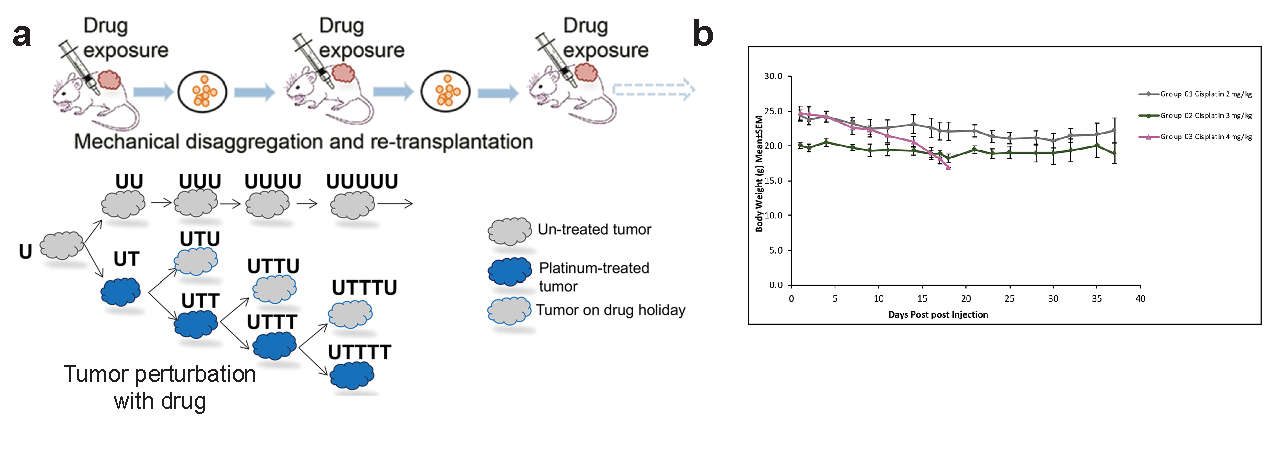
\includegraphics[width=\textwidth]{Figures/treatmentdesignMTD.pdf}
	
\caption[Experimental overview of TNBC PDX treated time series]
	{\small
	\textbf{Experimental overview of treatment design in TNBC PDX time series}
\textbf{(a)} Experimental design of cisplatin treatment in PDX.The residual tumour from one treated mouse was re-transplanted in the next (n=8). The solid blue colour represent cisplatin treated tumours \textit{(UT, UTT, UTTT, UTTTT)}; blue outlined in grey represents drug holiday \textit{(UTU, UTTU, UTTTU)}. Grey represent the untreated series \textit{(U, UU, UUU, UUUU, UUUUU)} \textbf{(b)} Mouse body weight graph recorded during \ac{MTD} evaluation of cisplatin in NRG mice (n=3 in each study cohort).}
	
	\label{fig:treatmentdesignMTD}
\end{figure}







\subsection{PDX tumour growth measurement curves} 
NRG mice received sub-cutaneous inoculation (SQ) of tumour cells (\SI{150}{\ul}) on day 0. 
The tumours were allowed to grow to palpable solid nodules.
Around 7-9 days after they are palpable, their size were measured with calipers every 3rd day. 
tumours were measured in two dimensions using a digital caliper and expressed as tumour volume in mm3; defined as: [volume= 0.52$\times$(Length)$\times$(Width)].
Under drug perturbation, the treated tumours in the first two cycles of treatment showed rapid growth reduction but in third cycle started showing non-responsive behaviour leading to total resistance in fourth cycle 




\section{Single cell whole genome sequencing and library construction with DLP+}

All libraries, including metrics on number of cells, average number of reads per cell and quality control metrics are listed in refsuptab{tab:omnibusMedians}.

\subsection{Creation of single cell suspensions from PDX}
Tumour fragments from PDX samples were incubated with a collagenase/hyaluronidase 1:10 (10X) enzyme mix (STEM CELL technologies, Catalog \#07912) in  \SI{5}{\ml} DMEM/F-12 with Glucose, L-Glutamine and HEPES (Lonza 12-719F)and 1\%BSA at \SI{37}{\degreeCelsius} with intermittent gentle pipetting up and down the sample every 30 min for 1 min, during the first hour with a wide bore pipette tip, 
and every 15-20 min for the second hour, followed by  centrifugation (1100 rpm, 5 min) and supernatant removal.
The tissue pellet was resuspended in \SI{1}{\ml} of  0.25 percent trypsin-EDTA (VWR CA45000-664) for 1 min, 
superadded by \SI{1}{\ml} of DNAse 1/dispase \SI{100}{\ul}/\SI{900}{\ul} (StemCell 07900,00082462) pipetted up and down 2 min, followed by neutralization with 2\% FBS in HBSS with 10 mM HEPES (STEMcells Catalog \#37150). 
This cell suspension was then passed through a \SI{70}{\micro\metre} filter to remove remaining undigested tissue and centrifuged for 5 min at 1100 rpm after topping it up to \SI{5}{\ml} with HBSS.
Single cells pellet  was resuspended in PBS + 0.04\% BSA (Sigma) in appropriate volume to achieve  $\approx$~1 million per ml concentration of cells for robot spotting for DLP+.

\subsection{Robot spotting of single cells into the nanolitre wells and library construction}
scWGS DLP+ library construction was carried out as described in \cite{laks2019clonal}. Briefly, single cell suspensions from cell lines and patient derived xenografts were fluorescently stained using CellTrace CFSE (Life Technologies) and LIVE/DEAD Fixable Red Dead Cell Stain (ThermoFisher) in a PBS solution containing 0.04\% BSA (Miltenyi Biotec 130-091-376) incubated at \SI{37}{\degreeCelsius} for 20 minutes. Cells were subsequently centrifuged to remove stain, and resuspended in fresh PBS with 0.04 percent BSA. This single cell suspension was loaded into a contactless piezo electric dispenser (sciFLEXARRAYER S3, Scienion) and spotted into the open nanowell arrays (SmartChip, TakaraBio) preprinted with unique dual index sequencing primer pairs. Occupancy and cell state were confirmed by fluorescent imaging and wells were selected for single cell copy number profiling using the DLP+ method \cite{laks2019clonal}. Briefly, cell dispensing was followed by enzymatic and heat lysis. After cell lysis, tagmentation mix 
(\SI{14.335}{\nano\liter} TD Buffer, \SI{3.5}{\nano\liter} TDE1, and \SI{0.165}{\nano\liter} 10\% Tween-20) in PCR water were dispensed into each well followed by incubation and neutralization. Final recovery and purification of single cell libraries was done after 8 cycles of PCR. Cleaned up pooled single-cell libraries were analyzed using the Aglient Bioanalyzer 2100 HS kit. Libraries were sequenced at UBC Biomedical Research Centre (BRC) in Vancouver, British Columbia on the Illumina NextSeq 550 (mid- or high-output, paired-end 150-bp reads), or at the GSC on Illumina HiSeq2500 (paired-end 125-bp reads) and Illumina HiSeqX (paired-end 150-bp reads). The data was then processed to quantification and statistical analysis pipeline \cite{laks2019clonal}.

\subsection{Identifying clones through phylogenetic analysis}
Using sitka we established the evolutionary relationships of cells in a PDX heterogeneous samples. To investigate cancer evolution we need to determine the abundance of subpopulations over time. To this end, we introduce \textbf{Lumberjack}, a tree-cutting algorithm that we used to define clonal subpopulations. In the output tree of \textbf{sitka}, cells are part of the terminal leaf nodes of the phylogenetic topology. We post-processed the inferred trees to identify clonal populations from major clades. When clonal populations are defined, their abundances were counted as a function of timeseries and these were used for fitness inference. 
Clones are constructed by identifying connected components (each a clade or a paraphyly) in the phylogenetic tree reconstruction. The tree is `cut' into discrete populations according to the following procedure
\subsubsection{Sitka Model}
\subsubsection{Lumberjack}



\section{Single cell RNA sequencing (scRNAseq)}
All libraries generated using 10x scRNAseq are listed in suptab{stab:tenx}.


\subsection{Processing of patient derived xenografts for scRNAseq data}
PDX tumours were harvested and mechanically disaggregated into small fragments to viably freeze them according to the protocol mentioned above. 
One of the viable frozen tumour vial was thawed and after washing out the freezing media, the tumour clumps and fragments were incubated with digestion enzymes as with DLP+ preparation. After complete dissociation with collagenase/hyaluronidase enzyme mix according to the protocol at \SI{37}{\degreeCelsius}, followed by briefly washing in 0.05\% trypsin-EDTA and resuspension in 0.04\% BSA in PBS. Dead cells were removed using the Miltenyi MACS Dead Cell Removal kit and cells were processed as previously described \cite{o2019dissociation}.
To avoid processing artifacts, dissociation methods and times were tightly controlled and for treatment and treatment holiday pairs, library construction was performed on the same chips. Single cell suspensions were loaded onto the 10x Genomics single cell controller and libraries prepared according to the Chromium Single Cell 3’ Reagent Chemistry kit standard protocol. 
Libraries were then sequenced on an Illumina Nextseq500/550 with 42bp paired-end reads, or a HiSeq2500 v4 with 125bp paired-end reads. 10x Genomics Cell Ranger 3.0 was used to perform demultiplexing, alignment and counting.




Library construction sample batch groupings are listed in 





{stab:tenx}.

